
\section{IME Architecture}
IME system is based on a Client-Server interaction: every compute node has a
Client side process intercepting IO communications that are sent to IME servers.
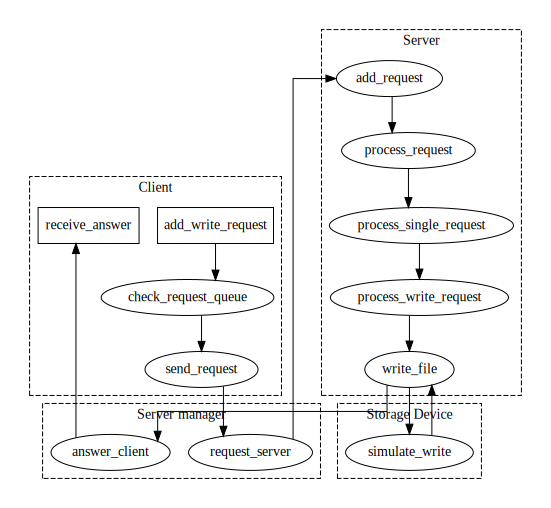
\includegraphics[width=\textwidth]{map.png}
The picture capture a possible configuration of IME:
\begin{itemize}
    \item 3 Clients with a single HDD each. These will generate the data that
        has to be stored in IME servers.
    \item a Network Fabric that interconnects every component of IME
    \item 2 SSDs per server, that can store data faster compared to the single
        client's HDD
\end{itemize}

Given the skeleton of the architecture, can be added or removed clients,
servers and disks for each one. This changes will end in different performances
that the simulator must be able to detect. \\
Part of the work is to inspect also different system layouts. The advantage of a
simulator is the ability to ensure the quality of a layout without the need to
test it for real, assuming the simulator is precise enough.
Every layout will be discussed in depth in the analysis section
(\ref{sys-analysis}).

\subsection{Network communication time}\label{netbuff}
Network communication is one of the main task that are committed in this system,
so we need an accurate model to represent it. \\
The parameters that determine the time elapsed in a network transaction are
\textit{latency} and \textit{bandwidth}. A file in theory is sent dividing
its size by the bandwidth available. In the real world we have to keep account also
the latency present inside the system: the smallest file will be sent
only after $<latency>$ amount of time. \\
From \cite{packet-size-ib} we know that the optimal packet size for
communication over infiniband is 1MB. \\
IME Client packs together requests smaller than this threshold and split bigger
files to achieve this communication pattern. This is further referred as
\textbf{Network Buffer}.  If requested explicitly, every request can be flushed
in order to complete a communication in case of remainders.  This set a domain
over the size of the packet sent: we always will have packets that are in the
interval $]0, 1024] KB$. The model should predict correctly the time required by
any network communication inside this interval. \\ In this case the only bond I
have are the 2 coordinates \\

\vspace{0.5cm}
\begin{tabular}{c | c}
    file size (KB) & time required \\ \hline
    0 & \textit{latency} \\ \hline
    1024 & \textit{1024KB / bandwidth}
\end{tabular}
\vspace{0.5cm}

These are respectively the worst and the best usage of the network. \\
I can obtain a more accurate model running some benchmarks on IME network, but
from a starting point I can rely on these 2 constraint. \\
Having the possibility to choose my interpolating function, I decided to use a
function with a diagonal limit, namely $\lim_{x \to +\infty} y(x) = +\infty$, that is a real behaviour
for every network. \\
The function of choice then is an \textit{hyperbole} adjusted to match the
specified coordinates. \\
\includegraphics[width=\textwidth]{diaglimit.png}


\subsection{Tokenized communication}
\subsection{Erasure coding for data loss} \label{pargroup}
In CPU caches whenever happens a cache miss, data is read from main memory
instead. No data can be potentially lost. In the worst case cache won't be
useful. \\ 
IME acts as a cache too but for the problem it is solving, there is no
communication between the of which it acts as a cache. This means that if data
is lost inside IME, it is permanently lost. IME has a system to overcome this
problem that is \textit{Erasure Coding}. \\
As it happens in RAID level 4, 5 and 6, what is stored in the disks is not just
data but also an added amount of data based on the original data. In case of 
loss of one piece of data, this missing part can be reconstructed comparing
remaining data and parity. \\
\includegraphics[width=\textwidth]{raid-level4.jpg} \\
For this correction system to work, we need to make associations between groups
of data that must be grouped together later when data loss happens. IME
considers a single block of data a Network Buffer (see \ref{netbuff}) and the
group that will contribute to data recovery as a \textbf{Parity Group}. \\
As an example, from the picture A1, A2, A3 and A$_p$ are individually a Network
Buffer. All of them grouped together makes a Parity Group. \\
The parity is generated by the client since the servers has only to keep track
about their status.



\subsection{Server Side file management}
\subsection{IO operations}
\begin{itemize}
    \item Sync
    \item Purge
    \item Erase
\end{itemize}
